\documentclass{beamer}					% Document class

\usepackage[english]{babel}				% Set language
\usepackage[utf8x]{inputenc}			% Set encoding

\mode<presentation>						% Set options
{
  \usetheme{default}					% Set theme
  \usecolortheme{default} 				% Set colors
  \usefonttheme{default}  				% Set font theme
  \setbeamertemplate{caption}[numbered]	% Set caption to be numbered
}


\usepackage{graphicx}					% For including figures
\usepackage{booktabs}					% For table rules
\usepackage{hyperref}					% For cross-referencing

\title{Monte Carlo Conformal Prediction for Hidden Markov Models}	% Presentation title
\author{Ghaleb Khalil, Andrew Wang}								% Presentation author
\institute{
University of Washington \\
STAT 538 - Statistical Learning \\
Instructor: Prof. Xinwei Shen
}					% Author affiliation
\date{March 9, 2026}							% Today's date	

\begin{document}

% Title page
% This page includes the informations defined earlier including title, author/s, affiliation/s and the date
\begin{frame}
  \titlepage
\end{frame}

% Outline
% This page includes the outline (Table of content) of the presentation. All sections and subsections will appear in the outline by default.
\begin{frame}{Outline}
\begin{enumerate}
    \item Problem Setting
    \item Computational Limitation
    \item Monte Carlo Approximation
    \item Theoretical Guarantees
    \begin{itemize}
        \item Unbiasedness
        \item Concentration Bound
        \item Coverage Preservation
        \item Asymptotic Convergence
    \end{itemize}
    \item Empirical Study
\end{enumerate}
\end{frame}

% The following is the most frequently used slide types in beamer
% The slide structure is as follows:
%
%\begin{frame}{<slide-title>}
%	<content>
%\end{frame}

\begin{frame}{Problem Setting}

\textbf{Goal:} Predict future hidden states of a Hidden Markov Model (HMM) with statistical guarantees.

\vspace{0.3cm}

Given observations
\[
Y_1,\dots,Y_T
\]

predict the future hidden state sequence
\[
X_{T+1:T+T_1}=(X_{T+1},\dots,X_{T+T_1})
\]

For a candidate sequence \(x\), compute the conformal p-value
\[
q(x)
\]

Construct the prediction set
\[
C_{1-\alpha}=\{x: q(x)\ge t\}
\]

such that
\[
P(X_{T+1:T+T_1}\in C_{1-\alpha})\ge 1-\alpha
\]

\end{frame}

\begin{frame}{Computational Limitation}

\textbf{Key issue:} The algorithm evaluates conformity scores for 
\textbf{all permutations of blocks}.

\vspace{0.4cm}

Cost per permutation:
\[
O(T_1 |X|^2)
\]

\vspace{0.3cm}

Number of permutations:
\[
|\Pi| = \frac{d!}{(d - T_1 - 1)!}
\]

Asymptotically,
\[
|\Pi| \approx d^{T_1+1}
\]

\vspace{0.3cm}

Total computational complexity:
\[
\mathbf{O(|\Pi|\,T_1|X|^2)}
=
\mathbf{O(d^{T_1+1}T_1|X|^2)}
\]

\vspace{0.4cm}

\textbf{Conclusion:} The algorithm becomes computationally infeasible for
large datasets.

\end{frame}

\begin{frame}{Monte Carlo Approximation}

\textbf{Idea:} Sample permutations instead of enumerating all permutations.

\vspace{0.2cm}

Exact conformal p-value (exhaustive computation):

\[
q(x) = \frac{1}{|\Pi|}\sum_{\pi \in \Pi} Z(\pi)
\]

\(Z(\pi)\in\{0,1\}\) indicates whether the permuted score exceeds the candidate score.

Monte Carlo estimator:

\[
\hat{q}_M(x) = \frac{1}{M}\sum_{m=1}^{M} Z(\Pi_m),
\qquad
\Pi_m \sim \text{Uniform}(\Pi)
\]

\vspace{0.1cm}

Computational cost reduction:
\[
O(|\Pi|)
\;\;\longrightarrow\;\;
O(M)
\]

\textbf{Key benefit:} Reduces computational cost from exponential to linear in the number of sampled permutations.

\end{frame}

\begin{frame}{Theoretical Guarantees: Unbiasedness}

\textbf{Result}

\[
\mathbb{E}[\hat{q}_M(x)] = q(x)
\]

\vspace{0.3cm}

\textbf{Tools used in the proof}

\begin{itemize}
\item Representation of the conformal p-value:
\[
q(x)=\frac{1}{|\Pi|}\sum_{\pi\in\Pi} Z(\pi)
\]
\item Uniform permutation sampling: \(\Pi_m \sim \text{Unif}(\Pi)\)
\item Linearity of expectation
\end{itemize}

\vspace{0.3cm}

\textbf{Interpretation}

The Monte Carlo estimator is unbiased for the exact conformal p-value.

\end{frame}

\begin{frame}{Theoretical Guarantees: Concentration Bound}

\textbf{Result}

\[
P\left(|\hat{q}_M(x)-q(x)|>\epsilon\right)
\le
2\exp(-2M\epsilon^2)
\]

\vspace{0.3cm}

\textbf{Tools used in the proof}

\begin{itemize}
\item \(Z(\Pi_m)\in\{0,1\}\) (bounded random variables)
\item i.i.d. permutation sampling: \(\Pi_m \sim \text{Unif}(\Pi)\)
\item Hoeffding's inequality
\end{itemize}

\vspace{0.3cm}

\textbf{Interpretation}

The estimator concentrates exponentially fast around the exact conformal p-value as the number of Monte Carlo samples \(M\) increases.

\end{frame}

\begin{frame}{Theoretical Guarantees: Coverage Preservation}

\textbf{Result}

\[
\mathbb{P}\big(X_{T+1:T+T_1} \in \hat C_{1-\alpha}\big)
\ge
1-\alpha - 2e^{-2M\epsilon^2}
\]

\vspace{0.3cm}

\textbf{Tools used in the proof}

\begin{itemize}
\item Exact conformal validity
\item Hoeffding concentration bound
\item Event decomposition and union bound
\end{itemize}

\vspace{0.3cm}

\textbf{Interpretation}

The Monte Carlo prediction set preserves conformal coverage,
with an error that vanishes exponentially fast as the number
of Monte Carlo samples \(M\) increases.

\end{frame}

\begin{frame}{Theoretical Guarantees: Convergence Rate}

\textbf{Result}

\[
\hat{q}_M(x) \to q(x) \quad \text{as } M \to \infty
\]

\vspace{0.3cm}

\[
|t-\alpha|
=
O\!\left(\sqrt{\frac{\log M}{M}}\right)
\]

\vspace{0.3cm}

\[
\hat C_{1-\alpha} \rightarrow C_{1-\alpha}
\]

\vspace{0.3cm}

\textbf{Tools used in the proof}

\begin{itemize}
\item Hoeffding concentration bound
\item Threshold analysis for the conformal set
\item Asymptotic limit \(M \rightarrow \infty\)
\end{itemize}

\vspace{0.3cm}

\textbf{Interpretation}

As the number of Monte Carlo samples increases, the approximate
prediction set converges to the exact conformal prediction set.

\end{frame}

\begin{frame}{Empirical Study (Work in Progress)}

\textbf{Experiments currently running}

\vspace{0.4cm}

Evaluation focuses on:

\begin{itemize}
\item Coverage accuracy of the conformal prediction set
\item Convergence of the Monte Carlo estimator \( \hat{q}_M(x) \)
\item Comparison with the exact conformal method
\item Computational efficiency as the number of permutations \(M\) increases
\end{itemize}

\vspace{0.3cm}

\textit{Goal: Validate the theoretical guarantees through simulation and empirical analysis.}

\end{frame}

\vspace{0.4cm}

\begin{frame}{Empirical Study (Work in Progress)}

Elapsed time and average elapsed time per future path using A100 GPU and 83.5GB RAM. Time efficiency improves dramatically past 10 periods of prediction.

\begin{figure}
    \centering
    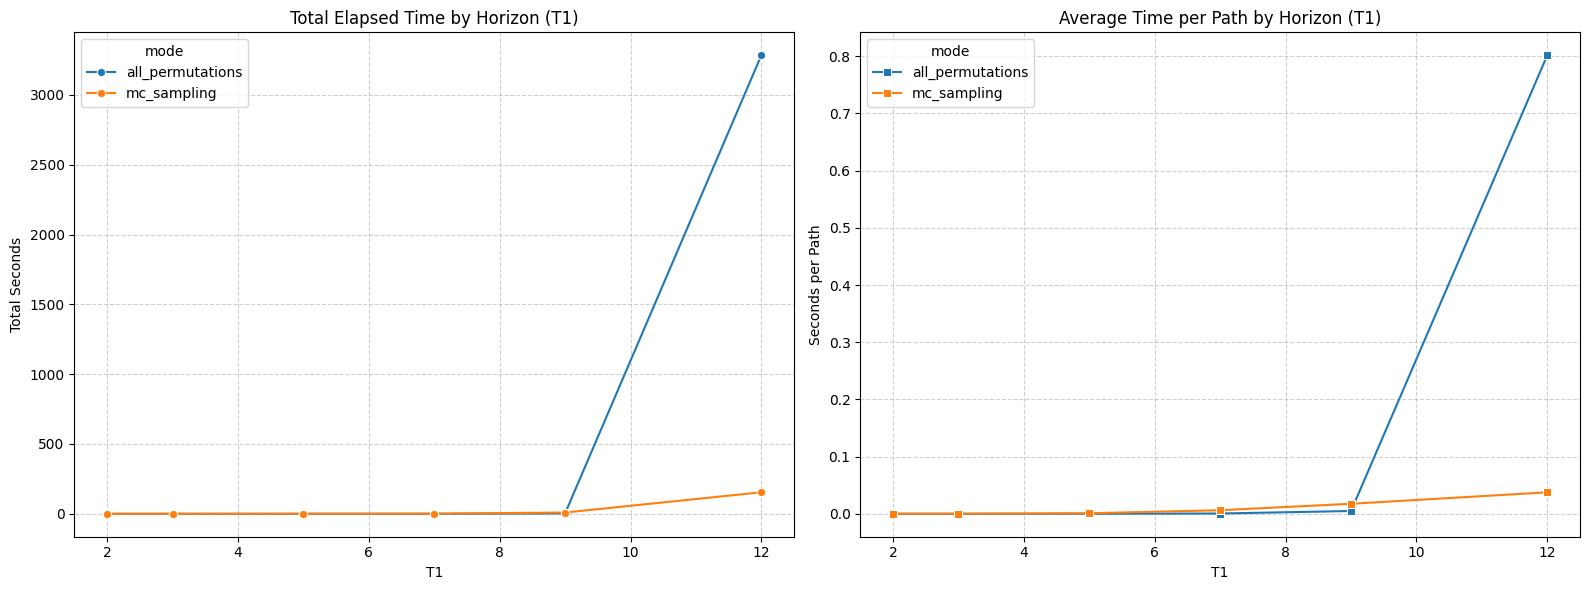
\includegraphics[width=1\linewidth]{Time efficiency.png}
    \caption{}
    \label{fig:timeefficiency}
\end{figure}
    
\end{frame}

\begin{frame}{Empirical Study (Work in Progress)}

Similarity of conformal sets at $\alpha = 0.1$. This is a visualization of the full permutation case.

\vspace{0.4cm}

\begin{figure}
    \centering
    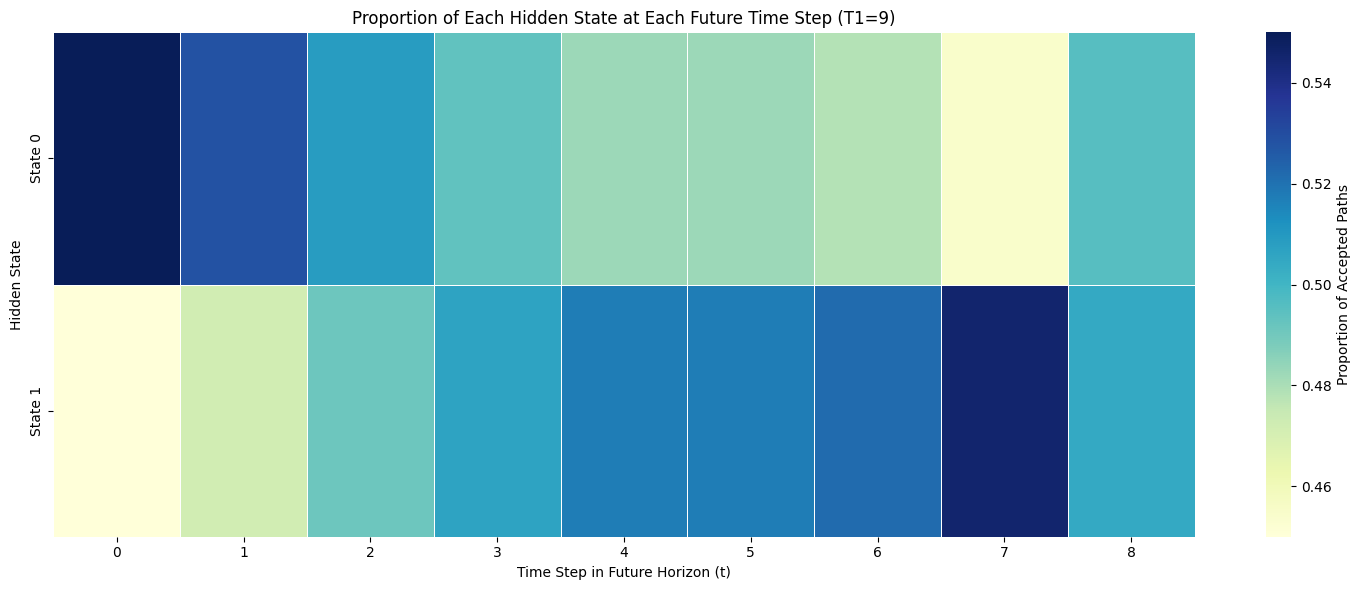
\includegraphics[width=1\linewidth]{C10_T.png}
    \caption{}
    \label{fig:timeefficiency}
\end{figure}
    
\end{frame}

\begin{frame}{Empirical Study (Work in Progress)}

And compare with this visualization of the MC sampling case.

\vspace{0.4cm}

\begin{figure}
    \centering
    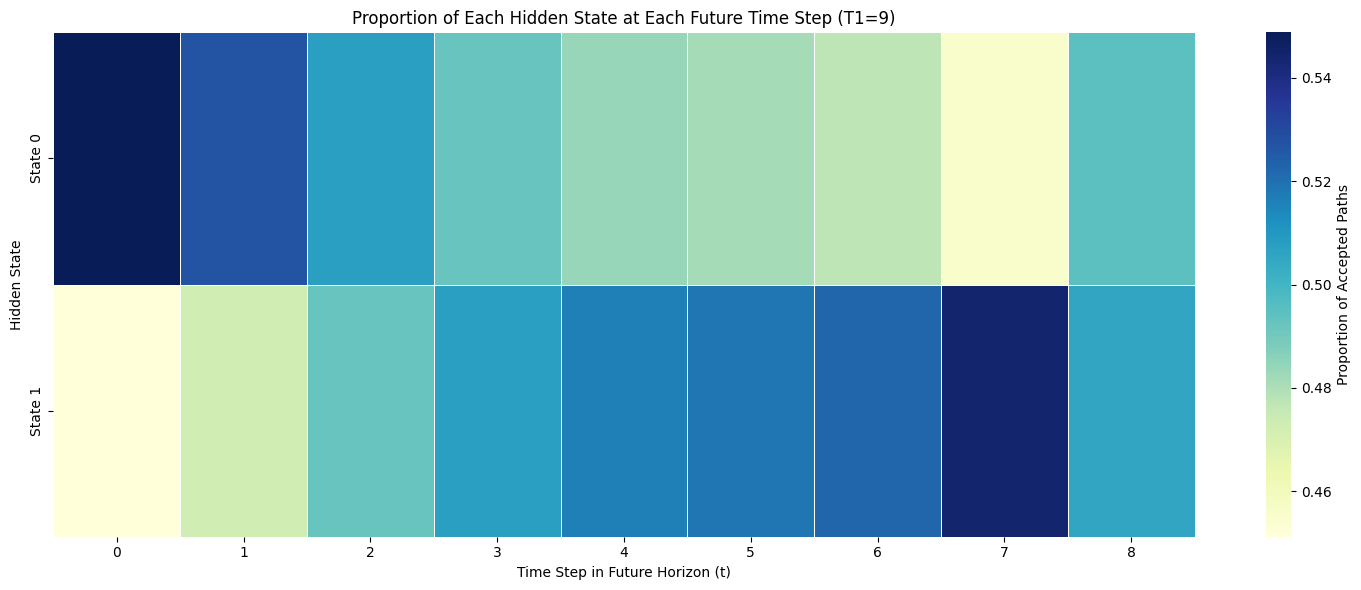
\includegraphics[width=1\linewidth]{C10_F.png}
    \caption{}
    \label{fig:timeefficiency}
\end{figure}
    
\end{frame}

\end{document}
